% NIP - project documentation
% Mikko Korpela, Antti Rasinen, Janne Toivola 2004
% $Id: doc.tex,v 1.1 2010-11-24 12:10:25 jatoivol Exp $

\documentclass[12pt,a4paper]{report}
\bibliographystyle{unsrt}
\setlength{\topmargin}{0mm}
\setlength{\oddsidemargin}{0mm}
\setlength{\textheight}{22cm}
\setlength{\textwidth}{16cm}
\usepackage[T1]{fontenc}
\usepackage[latin1]{inputenc}
\usepackage[english]{babel}
\usepackage[dvips]{graphicx}
\usepackage{amsmath}
\usepackage{subfigure}
\usepackage{tocbibind}
\usepackage{fancyvrb}
\usepackage{times}
\usepackage{hyperref}
%\newcommand{\argmax}{\mathrm{argmax}}
%\newcommand{\argmin}{\mathrm{argmin}}
%\newcommand{\define}{\stackrel{\mathrm{def}}{=}}


% Reminder about the style so far: 
% - C data types     {\it unsigned long}
% - code examples    \texttt{this = is_an(example);}
% - file names       \texttt{filename.txt}
% - defined stuff    \textbf{A_DEFINED_VALUE}
% - parameter names  \textbf{parameter}
% ...
% Try to keep it consistent...

\newcommand{\cdatatype}[1]{{\it #1}}
\newcommand{\examplecode}[1]{\texttt{#1}}
\newcommand{\cfilename}[1]{\texttt{#1}}
\newcommand{\cdefine}[1]{\textbf{#1}}
\newcommand{\cparameter}[1]{\textbf{#1}}
\newcommand{\cstructfield}[1]{\textbf{#1}}
\newcommand{\cfunction}[1]{\texttt{#1}}


%--------------------
% Place this in the preamble of your LaTeX file:
% (c) Jaakko Hollmen, 2002

\usepackage{ifthen}

% Declare the variable doublespaced
\newboolean{doublespaced}

% Comment one of the following lines to either select
% doublespaced or singlespaced:
\setboolean{doublespaced}{false}
%\setboolean{doublespaced}{true}

\ifthenelse{\boolean{doublespaced}}
{
  % Double spaced text if variable "doublespaced" is true:
  \renewcommand{\baselinestretch}{1.5}
  \normalsize % necessary to execute the previous thing
}
{
  % This is to be executed if doublespace is false:
  % else = do nothing
}
%--------------------

\title{NIP}
\author{Antti Rasinen 49569V}
\author{Mikko Korpela 54919L}
\author{Janne Toivola 55173U}
\begin{document}

\pagestyle{empty}
\setlength{\parindent}{0mm}
\setlength{\parskip}{3mm}

\large
\textbf{The NIP project}\\

\vspace{45mm}

\begin{centering}
\huge
\textbf{System description}\\ % Any better names for this?
\end{centering}

\parbox{5cm}{\ }
\parbox{1em}{\vskip8cm}

\normalsize
\vspace{5mm}
\begin{tabbing}
The Team:\= Antti Rasinen\\
         \> Mikko Korpela\\
         \> Janne Toivola\\
\vspace{5mm}

\end{tabbing}
%----------------------
Date: \today
%----------------------
\eject\newpage

\pagestyle{plain}

\tableofcontents

%\newpage
%
%\listoffigures


\newpage
\chapter{General description}
This document describes a software library developed by the authors at the
laboratory of computer and information science (CIS) at Helsinki University
of Technology. The software library provides tools for Bayesian inference
within the domain of multivariate discrete time series...
% What?


\section{Overview}
The implementation can be seen as a set of layers divided in levels of
abstraction (see Fig.~\ref{fig1}). The lowest level of computation is done
with so-called potentials and therefore the abstract data type (ADT) 
{\it potential} is used throughout the system. Another common data type is 
{\it variable} which contains information e.g. about the name of a variable 
and its states.
%
\begin{figure} [!ht]
  \begin{center}
    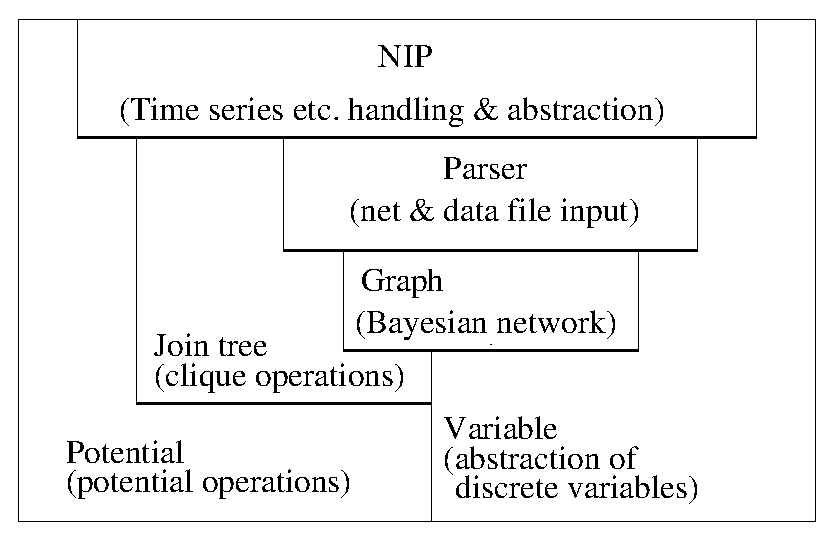
\includegraphics[width=110mm]{layers.eps}
    \caption{Abstraction layers of the system}
    \label{fig1}
  \end{center}
\end{figure}

Files {\it Graph.h} and {\it Graph.c} contain part of the software
responsible for Bayesian network representation and transformation into a
so-called {\it join tree}. Various operations for handling join trees is
located in {\it clique.h} and {\it clique.c}. Abstractions provided by
potential, clique, graph and variable subsystems are used by the 
{\it parser} subsystem for reading models and data from input files. 
Finally the {\it nip} subsystem (files nip.h and nip.c) provides
abstraction for time series and most of the other things mentioned above.

The following sections will explain each of the subsystems in close
detail. Probably the most important parts for the user of this software
library are the ones describing variables and NIP abstractions.


\newpage
\chapter{Subsystem descriptions}
% The nasty details

\section{Variables}
\subsection{General}
All the variables $V$ are assumed to be discrete and have a certain
number of states: $c_V$ which is also known as the {\it cardinality} 
of the variable $V$. Thus the probability distribution i.e. likelihood 
$\lambda_V$ of a variable $V$ can be represented as a table of values 
and the size of the table is $c_V$. Furthermore, the sum of the values 
in the table equals one:
\begin{equation}
\sum_{v=0}^{c_V-1} \lambda_V[v] = 1.
\end{equation}

The main idea of the whole system is to describe dependencies between
variables. This is achieved by {\it graphs}, {\it potentials}, and 
{\it cliques} presented in the following sections. Shortly, the variables
are said to be {\it children} depending on their {\it parent} variables. A
variable $V$ and its parents $\mathbf{\Pi}_V$ form a set of variables 
$\mathbf{F}_V$ naturally called the {\it family of V}. There's more about
the quantitative relationship in the following sections.

\subsection{Functionality description}

\subsubsection{The data structure}
The data type \cdatatype{variable} defined in \cfilename{variable.h} 
is a pointer to a struct which has the following fields: 
\begin{description}
\item[symbol] is a short string used for identifying the variable. Maximum
  length is defined as \cdefine{VAR\_SYMBOL\_LENGTH} in 
  \cfilename{variable.h}. To ensure the correct operation of the system, the 
  symbol should be unique.

\item[name] is usually a longer name to describe the variable: it is
  called {\it label} in the Hugin net language files. This is NOT used for 
  identification of the variables and it doesn't need to be unique. 
  The maximum length is defined as \cdefine{VAR\_NAME\_LENGTH} in 
  \cfilename{variable.h}.

\item[statenames] is an array of strings containing names for all
  possible states of the variable. The identification of data relies on
  these strings. The size of the statenames array i.e. number of
  strings should be the same as the number of states indicated by
  cardinality field described below.

\item[cardinality] is a positive integer which tells how many states
  the variable can have. It plays an important role in all calculations
  so it better be correct: the value is not meant to be altered.

\item[id] is an \cdatatype{unsigned long} used for identification
  inside the system. It is set automatically by the \cfunction{new\_variable} 
  function and should not be tampered after that.

\item[likelihood] is a \cdatatype{double} array describing the probability
  distribution of the states of the variable. It is used only for
  entering evidence into the system and likelihood arrays of the latent
  variables remain filled with ones. Size of the array equals
  cardinality, of course.

\item[previous] is used for describing the repetitive structure in
  timeslice models. It is a pointer to the variable which this variable
  will replace in previous timeslice. The pointer is \cdatatype{NULL} if 
  the model has no repetitive structure or dependencies between time steps.

\item[next] is a same kind of pointer as \cstructfield{previous} above, 
  but this one tells which variable will be replaced in the next timeslice.
  The \cstructfield{previous} and \cstructfield{next} pointers should be 
  symmetrical i.e. if \examplecode{a->next == b} then 
  \examplecode{b->previous == a}.

\item[parents] is an array of references to the parent variables 
  (\examplecode{variable[]}) or a null pointer if there are no parents.

\item[num\_of\_parents] is a positive \cdatatype{integer} which tells the 
  number of parents and thus the size of the \cstructfield{parents} array.

\item[family\_clique] is a void pointer for so-called memoization of family
  cliques of variables. The pointer is initially NULL and is set only when 
  the family clique is found the first time.

\item[family\_mapping] is an integer array telling which variables of the
  clique belong to the family and in which order. This is only a
  memoization trick for some join tree operations.

\item[pos\_x] is an integer describing horizontal position of the graph
  node on computer display. This is also known as the {\it node position}
  in Hugin net files.

\item[pos\_y] is an integer describing vertical position of the graph node
  on computer display. (a.k.a. the {\it node position} in Hugin net files)

\item[mark] is a field of type \cdatatype{char}. It can be used by
  algorithms like DFS or the one that generates artificial data 
  according to a model.
\end{description}

\cfilename{variable.h} provides also data types for implementing lists of
variables. Both \cdatatype{varlink} and \cdatatype{variable\_iterator} are
pointers to structs which contain following fields:
\begin{description}
\item[data] is the variable (i.e. pointer to a variable struct) 
contained by the list element.

\item[fwd] is a pointer to the next element in the list or \cdatatype{NULL}
at the end of the list.

\item[bwd] is a pointer to the previous element in the list or 
\cdatatype{NULL} at the beginning of the list.
\end{description}
Variable iterators are meant to be used the same way as list iterators
in Java: you can get the next element contained by the list by just 
calling \examplecode{next\_variable(iterator)}. On the other hand, iterators
are NOT meant to be the only reference to a list because it will
advance in the list, pointing always to the next element and eventually
be a null pointer.


\subsubsection{The functions}
The functions provided in \cfilename{variable.c} are
%The interface + how the stuff works...
\begin{description}
\item[new\_variable(symbol, name, states, cardinality)] creates a variable
  identified with the \cparameter{symbol} string. The \cparameter{name}
  string will be copied as the name field of the new variable. Both the
  \cparameter{symbol} and \cparameter{name} strings may be truncated to the
  allowed length. The states of the new variable will be named according to
  the given string array \cparameter{states}.  All the given strings are
  copied, so remember to free them after they become useless. Initially, the 
  variable will not have parents, so you have to set them separately.

\item[copy\_variable(v)] returns an exact copy of the
  variable~\cparameter{v}. Note that also the id~field is copied and
  consequently there may not be two copies of the same variable in the same
  model.

\item[free\_variable(v)] frees the memory allocated for the
  variable~\cparameter{v}.

\item[equal\_variables(v1, v2)] returns 0 if either of the variables
  are null. Otherwise it will tell if the variables have equal id fields
  or not.

\item[get\_id(v)] will return the unsigned long id field of the
  variable~\cparameter{v}.

\item[mark\_variable(v)] marks the variable~\cparameter{v}. You can use
  this if some algorithm needs to know which variables have been dealt
  with.

\item[unmark\_variable(v)] clears the mark for the variable~\cparameter{v}.

\item[variable\_marked(v)] tells if the variable~\cparameter{v} is marked
  or not (returns the integer 0 if not).

\item[get\_symbol(v)] returns the symbol of the variable~\cparameter{v}. It
  will not make a copy of the string so don't mess with the contents.

\item[get\_stateindex(v, state)] tells the place of the string
  \cparameter{state} in the state name array of the
  variable~\cparameter{v}. This index can be used for interpreting various
  arrays describing probability distributions. 

\item[total\_num\_of\_vars()] is used only for aiding the Hugin net
  language file parser to return the total number of newly created
  variables. All the variables (created with the \cfunction{new\_variable}
  function) are accumulated in a list and this function can tell the size of
  that list.

\item[get\_first\_variable()] gives the first element in the list of newly
  created variables mentioned above.

\item[get\_last\_variable()] gives the last element in the list of newly
  created variables mentioned above.

\item[reset\_variable\_list()] will replace the list of recently created
  variables with \cdatatype{NULL} and set the size of the list to zero. This
  is used only for resetting the list after copying the list pointer to a new
  model. Otherwise all the models would share the same list of parsed
  variables.

\item[next\_variable(it)] will give the next variable pointed by the
  variable iterator~\cparameter{it} and advance the pointer to the next
  variable in the list. The function returns \cdatatype{NULL} if the iterator
  runs out of variables.

\item[get\_parser\_variable(symbol)] aids the net language parser to find a
  variable, identified by the \cparameter{symbol} string, in the list of
  newly created variables.

\item[get\_variable(vars, nvars, symbol)] searches the \cdatatype{variable
  array}~\cparameter{vars} for a variable identified by the string
  \cparameter{symbol}. Also the size of the array has to be specified as the
  \cdatatype{integer}~\cparameter{nvars}.
  
\item[update\_likelihood(v, likelihood)] will set the likelihood array of
  variable~\cparameter{v} according to the given double array
  \cparameter{likelihood}. Size of the given array should be the same (or
  more) than the cardinality of the variable.

\item[reset\_likelihood(v)] fills the likelihood array of the
  variable~\cparameter{v} with ones. This means that the likelihood of the
  variable states will be uniform.

\item[number\_of\_values(v)] returns the cardinality of the
  variable~\cparameter{v}. It is the exact number of states the variable has
  and will always have.

\item[number\_of\_parents(v)] tells how many parents the
  variable~\cparameter{v} has.
  
\item[set\_position(v, x, y)] will set the integer position
  values~\cparameter{x} and \cparameter{y} of the variable~\cparameter{v}.

\item[get\_position(v, x, y)] will write the position values of the
  variable~\cparameter{v} into the integers referenced by the pointers 
  \cparameter{x} and \cparameter{y}.

\item[set\_parents(v, parents, nparents)] sets the parents for the
  variable~\cparameter{v} by copying the references from the
  \cparameter{parents}, which is an \cdatatype{array of variables}. 
  Size of the array must be specified by the \cparameter{nparents} 
  \cdatatype{integer}.

\item[get\_parents(v)] returns a reference to the parents of the 
  variable~\cparameter{v}. After you get the pointer to the array of 
  parents, DO NOT alter the content of the array. Note that the size of the
  array can be found out with the \cfunction{number\_of\_parents} function.

\item[set\_prior(v, prior)] sets the prior probability distribution for the 
  variable~\cparameter{v} according to the given \cdatatype{double array} 
  \cparameter{prior}. The array must have one element for each of the
  states of the variable. Old prior array will be de-allocated if it exists
  and the given array \cparameter{prior} is copied.

\item[get\_prior(v)] gives a base pointer to the \cdatatype{double array}
  describing the prior distribution of given variable \cparameter{v}.
  Don't mess with the contents of the array unless you need to alter the 
  prior distribution.
\end{description}


\subsection{Other possibilities}
The Hugin net language parser is made with Bison and consequently the
\cfunction{yyparse} function is not able to return a list of variables
etc. This makes it awkward to pass the results of parsing to the rest of
the program. Our solution is to create a list of parsed variables in
\cfilename{variable.c} by appending every newly created variable to it. The
list could also be at \cfilename{parser.c} in order to avoid having weird
functions like \cfunction{get\_parser\_variable}.

% length limitations of symbols, variable and state names?
We decided to have limitations for the lengths of variable symbols, labels
and state names. This made implementation a bit easier and limits the time
used for various comparison operations. This can also produce troubles in
the case that two variables have very long and almost identical names or
symbols. Truncating the length of variable symbols would then cause the
variables to be treated equal.


\newpage
\section{Graphs}
\subsection{General}

In graphical models the graphical layout describes independence and
conditional independence between variables. This is exploited to
obtain a computationally efficient factorisation of the joint
probability distribution. 

The purpose of the graphical analysis is to find an optimal set of
clusters in the graphical model that has the join tree property. These
clusters are later merged into a join tree. This tree is then used for
the actual inference.

The main steps in the graphical analysis process are moralisation and
triangulation. Put simply, moralisation means that any nodes that have
a common child are connected. Furthermore, all directed links are
replaced with undirected links. The resulting graph is called a {\it
(undirected) moral graph}. 

This graph is then triangulated. The triangulation process also
extracts the cliques used to build the join tree.  There exist several
triangulations for a given graph; we are interested in a triangulation
that is optimal in the sense of adding the least edges\footnote{If
there is more than one optimal solution, further constrains may be
introduced. For example, for memory efficiency we prefer the solution
that generates the smallest potential tables.} to the moral
graph. Finding such a triangulation is an NP-hard problem, but there
exist heuristics that give nearly optimal results.  The triangulation
algorithm is the one presented in \cite{huang1994}.

The \cdatatype{Graph} is implemented via an adjacency graph. The
interface is designed to hide the implementation details. The
\cdatatype{Heap} datatype used in the triangulation stage contains a
\cdatatype{Graph}-like datatype and could possibly be refactored.


\subsection{Functionality description}
%The interface + how the stuff works...
\subsubsection{The data structures}
The data type \cdatatype{Graph} defined in \cfilename{Graph.h} is a
struct which has the following fields:
\begin{description}
\item[adj\_matrix] is an $n\times n$ adjacency matrix for the
graph. The size $n$ is specified when the graph is first constructed
and it is stored in the variable \cparameter{size}. The matrix is
implemented as a simple array. For this reason it is manipulated via
the macro \cparameter{ADJM}.
\item[variables] is an array of variables associated with this graph.
\item[size] is the number of variables in the \cdatatype{Graph}.
\item[var\_ind] is an internal array of variables. Used for
performance reasons.
\item[min\_id] The smallest \examplecode{id} of a variable associated
with the graph. Used internally for better performance.
\item[max\_id] The largest \examplecode{id} of a variable associated
with the graph. Used internally for better performance.
\item[top] is an internal counter used when adding variables. 
\end{description}


\subsubsection{The functions}

The functions provided in \cfilename{Graph.c} are:

\begin{description}
\item[new\_graph(n)] creates a new graph with memory reserved for
  \cparameter{n} variables. Returns a pointer.
\item[copy\_graph(G)] creates a copy of the graph \cparameter{G}.
\item[free\_graph(G)] frees the memory reserved for the graph
  \cparameter{G}.
\item[get\_size(G)] returns the number of variables in the graph
  \cparameter{G}.
\item[get\_variables(G)] returns the variables in the graph
  \cparameter{G} as an array.
\item[get\_graph\_index(G, v)] returns the index of the variable
  \cparameter{v} in the internal array of the graph \cparameter{G}.
\item[get\_neighbours(G, v\_array, v)] returns the number of
  neighbours of variable \cparameter{v} in graph \cparameter{G}. The
  neighbours will be stored in the array \cparameter{v\_array}, which
  {\it must be large enough}. No variable can have more neighbours than
  $n-1$, where $n$ is the number of variables in \cparameter{G}.
\item[is\_child(G, v1, v2)] will return \examplecode{True} when
  variable \cparameter{v2} is a child of variable \cparameter{v1} in
  the graph \cparameter{G}.
\item[add\_variable(G, v)] adds a new variable \cparameter{v} to the
  graph \cparameter{G}. You must add as many variables as you specified
  when creating \cparameter{G}.
\item[add\_child(G, v1, v2)] adds an edge to graph \cparameter{G}
  from variable \cparameter{v1} to variable \cparameter{v2}, ie. makes
  \cparameter{v2} a child of \cparameter{v1}.
\item[find\_cliques(G, cp)] finds cliques in \cparameter{G} and
  stores them in the clique-array \cparameter{*cp}
  \footnote{Type of
    \examplecode{cp} is \cdatatype{clique**}, ie. it is a pointer to such
    an array. It need not be initialized.}. Returns the number of elements
  in the array.
\item[make\_undirected(G)] returns an undirected copy of Graph
  \cparameter{G}.
\item[moralise(G)] returns a moralised copy of graph \cparameter{G}.

\end{description}

\subsection{Notes on Implementation}

The above discussion describes only the interface of the
\cdatatype{Graph} module. Some data structures used internally by the
\cdatatype{Graph} module are summarily described here. The explanation
is mostly aimed at those planning to modify the module.

\subsubsection{Heap}

The \cdatatype{Heap} is used to keep the potential cliques in a sorted
data structure. Any search structure would suffice here; the heap is
probably the most efficient.

This step requires a dynamically updatable \cdatatype{Heap}. The
weights in neighbouring nodes change when the minimum weight node is
removed. This also means that the heap implementation must be tied in
with the \cdatatype{Graph}. This has led to number of tradeoffs and
possible pitfalls.
 
% XX


\subsubsection{cls2clq}

The \cdatatype{cls2clq} module is used to convert a list of clusters
to an array of cliques. In addition to a simple list implementation,
it also includes a method to check whether a given set of variables
(ie. a cluster) is a subset of a cluster already in the
list\footnote{There is no need to check for supersets; the items in
the list contain nodes that are then removed from the graph and thus
cannot occur in later clusters.} and a method for the list-to-array
conversion.

The list used in this implementation could be replaced with a generic
list data type.

\subsection{Other possibilities}

From efficiency standpoint, the approach presented in \cite{huang1994}
and suitable for production use.

If efficiency is not the main concern, eg. in prototyping situations,
some simplifications can be made. For example, the heap data structure
in the triangulation phase can be replaced with a list or array and a
linear search.

The interface is not as smooth and polished as it could be. It is also
not very flexible. For example you have to know the number of
variables when constructing the graph; the system should be able to
dynamically add new variables 'on the go'. However, such functionality
can be introduced with a wrapper, if desired.


\newpage
\section{Potentials}
\subsection{General}
As probability distributions of single variables are implemented as tables,
probability distributions relating to multiple discrete variables can be
represented as multidimensional tables. For example, if the variable~$X$
depends on a set of variables $\mathbf{Y}=$ $\{Y_1,\dots,Y_{N-1}\}$, the
dependency can be described quantitatively by the probability distribution
$P(X|\mathbf{Y})$.  Another example could be a joint distribution
$P(\mathbf{Z})$ of the variables $\mathbf{Z}=\{Z_1,\dots,Z_N\}$. These kind
of distributions can be thought as functions from the N-dimensional space
(formed by the variables $\{X\} \cup \mathbf{Y}$ or~$\mathbf{Z}$) to a real
number $p \in [0,1]$. Since the variables have a discrete and finite set of
states, the function can be viewed as an N-dimensional table
$\phi_\mathbf{Z}$ containing the real numbers corresponding to the
probabilities. As an example, the value $P(A=a_0, B=b_3, C=c_5)$ is found
in a multidimensional table $\phi_\mathbf{Z}$ as
$\phi_{\mathbf{z}={0,3,5}}$ or as \examplecode{P[0][3][5]} in a program.

There are two kinds of operations on potentials: marginalisation and
multiplication. Marginalisation is basically for reducing the number of
dimensions of a potential by calculating sums over the unnecessary
variables. For example, if $\mathbf{X} \subseteq \mathbf{Z}$,
$P(\mathbf{X})$ can be calculated from $P(\mathbf{Z})$ by summing over
$\mathbf{Z} \setminus \mathbf{X}$ and similarly
\begin{equation}
\phi_\mathbf{X} = \sum_{\mathbf{Z} \setminus \mathbf{X}} \phi_{\mathbf{Z}}.
\label{potentialmarginalisation}
\end{equation}
Which means that if we have $\mathbf{Z} = \{X, Z_2, Z_3\}$, then
\begin{equation}
\phi_X = \sum_{Z_2,Z_3} \phi_{\mathbf{Z}} \\
\Leftrightarrow \phi_X[i] = \sum_{j=0}^{c_{Z_2}-1}
\sum_{k=0}^{c_{Z_3}-1} \phi_\mathbf{Z}[i][j][k], \forall i \in [0,c_X-1]
\end{equation}

The multiplication operation has the same kind of idea: a potential can
be weighted with another one by multiplying suitable elements one by one.
Again, if we have $\mathbf{X} \subseteq \mathbf{Z}$, we may assign
\begin{equation}
\phi_\mathbf{Z} \leftarrow \phi_\mathbf{X} \phi_\mathbf{Z}.
\end{equation}
As an example, when $\mathbf{Z} = \{X, Z_2, Z_3\}$, the assignment
\begin{equation}
\phi_\mathbf{Z}[i][j][k] \leftarrow \phi_\mathbf{Z}[i][j][k]*\phi_X[i]
\label{potentialmultiplication}
\end{equation}
is done for all combinations of 
$(i,j,k) \in [0,c_X-1]\times[0,c_{Z_2}-1]\times[0,c_{Z_3}-1]$.

From the implementation point of view, one of the most important
notions is that an element in a multidimensional table can be referenced 
by a ``flat index'' also. For example, if we assume that the first index of 
an array is the least significant one and $\mathbf{X} = \{X_1,X_2\}$, then 
\begin{itemize}
\item $\phi_\mathbf{X}[0] = \phi_\mathbf{X}[0][0]$, 
\item $\phi_\mathbf{X}[i] = \phi_\mathbf{X}[i][0]$, if $i<c_{X_1}$,
\item $\phi_\mathbf{X}[i] = \phi_\mathbf{X}[i-c_{X_1}][1]$, if 
  $c_{X_1} \leq i < 2c_{X_1}$ etc.,
\item $\phi_\mathbf{X}[c_{X_1}] = \phi_\mathbf{X}[0][1]$, and 
\item $\phi_\mathbf{X}[c_{X_1}*c_{X_2}-1] = 
  \phi_\mathbf{X}[c_{X_1}-1][c_{X_2}-1]$, which is the last element. 
\end{itemize}


\subsection{Functionality description}

\subsubsection{The data structure}
The data type \cdatatype{potential} defined in \cfilename{potential.h} is a
pointer to a struct which contains the following fields:
\begin{description}
\item[size\_of\_data] is an \cdatatype{integer} telling the total number of
elements in the potential. It must be the product of all the elements in
the \cstructfield{cardinality} array (or one if the number of variables
equals zero).

\item[cardinality] is an array of \cdatatype{integers}. The integers are
the cardinalities of each variable the potential is related to. Thus the
size of the array must be the same as the number of variables. Also the
order of the cardinality array is significant because the variables are
assumed to have a certain order.

\item[num\_of\_vars] is an \cdatatype{integer} which tells the number of
variables associated with the potential.

\item[data] is the \cdatatype{double array} describing a probability
distribution of the associated variables. The size of this array is in the
\cstructfield{size\_of\_data} field. The data in the array is arranged
according to the order of the corresponding variables: the variable which
has its cardinality first in the \cstructfield{cardinality} array is
considered least significant in the sense of placing a value in the
\cstructfield{data} array.
\end{description}


\subsubsection{The functions}
The functions provided for manipulating \cdatatype{potentials} are 
placed in \cfilename{potential.c} and are as follows:
\begin{description}
\item[make\_potential(cardinality, num\_of\_vars, data)] creates a
  potential struct according to the parameters and returns a pointer to
  it. The resulting potential will have its cardinalities of variables set
  according to the given \cparameter{cardinality} array by copying the
  elements in it. The number of associated variables is given as the integer
  \cparameter{num\_of\_vars}.
  
  The \cparameter{data} parameter can be a null pointer or a
  \cdatatype{double array} of the size equal to the product of the
  cardinalities of the variables. In case of a null pointer, the potential
  will be initialised to uniform distribution. Otherwise the contents of the
  \cstructfield{data} array in the potential struct will be copied from the
  given \cparameter{data} array.
  
\item[free\_potential(p)] frees the memory allocated for the
  potential~\cparameter{p}.
  
\item[get\_pvalue(p, indices)] retrieves the possibly non-normalised
  probability of the configuration of variables, described by the
  \cdatatype{integer array} \cparameter{indices}, from the
  \cdatatype{potential}~\cparameter{p}. The \cparameter{indices} array tells
  which value each of the associated variables are assigned: $n-1$ in the
  array corresponds to the $n$:th value of the variable.  The
  \cparameter{indices} must be in the same order as the corresponding
  variables and their cardinalities in the potential~\cparameter{p}.
  
\item[set\_pvalue(p, indices, value)] sets a \cdatatype{double}
  \cparameter{value} in the \cdatatype{potential}~\cparameter{p} the same way
  as \\ \cfunction{get\_pvalue(p, indices)} retrieves it.  (See the
  description above.)
  
\item[inverse\_mapping(p, flat\_index, indices)] transforms a so-called
  flat index into the \cdatatype{integer array} \cparameter{indices}
  according to the \cdatatype{potential}~\cdatatype{p}.  A flat index is an
  index used for addressing data in the potential and is therefore an integer
  between \examplecode{0} and \examplecode{p->size\_of\_data - 1}
  inclusive. Shortly, this function is made for finding out which
  configuration of states of the variables corresponds to each element in the
  potential. Note that the \cparameter{indices} array is not allocated by the
  function.
  
\item[general\_marginalise(source, destination, mapping)] is one of the
  most useful functions since it computes the marginalisation i.e. a sum over
  the variables not being indicated by the given \cdatatype{integer array}
  \cparameter{mapping} and places the result in the given
  \cparameter{destination} potential. To make any sense, the number of
  associated variables in \cparameter{source} must be greater than in
  \cparameter{destination}.
  
  The \cparameter{mapping} array tells which variable in \cparameter{source}
  corresponds to each of the variables in \cparameter{destination}. It
  consists of indices ranging from \examplecode{0} to
  \examplecode{source->num\_of\_vars - 1} inclusive.  The $n$'th variable of
  destination potential corresponds to the $mapping[n]$'th variable in the
  source potential. Size of the array must equal the number of variables
  associated with the destination potential.  Note that the result of
  marginalisation is not normalised.
  
\item[total\_marginalise(source, destination, variable)] can be used for
  finding out the probability distribution of a single variable according to
  the \cparameter{source} potential. The function is similar to the
  \cfunction{general\_marginalise} but the user must indicate which one of
  the variables is left unmarginalised. The parameter \cparameter{variable}
  is an \cdatatype{integer} ranging from \examplecode{0} to
  \examplecode{source->num\_of\_vars - 1} inclusive. Zero indicates the first
  variable in the potential.
  
  Another difference arises from the fact that the probability distribution
  of a single variable fits into a one-dimensional array.  The place to put
  the resulting \cdatatype{double array} (\cparameter{destination}) is given
  to the function as one of the parameters. Size of the array must be equal
  (or greater) to the cardinality of the desired variable, so remember to
  allocate one before calling this function. Note that the result of
  marginalisation is not normalised.
  
\item[update\_potential(numerator, denominator, target, mapping)]
  implements the multiplication of potentials. The function simply multiplies
  the elements of the \cparameter{target} potential with the corresponding
  elements in the \cparameter{numerator} potential. At the same time, the
  function is able to divide the \cparameter{target} potential with the
  optional \cparameter{denominator} potential. If no division is needed,
  \cparameter{denominator} can be \cdatatype{NULL}.  The
  \cparameter{numerator} and \cparameter{denominator} potentials are left
  unchanged by the function.
  
  The function is made for multiplying a clique potential with the old
  and new sepset potentials. It is assumed that the variables associated with
  the multiplier potentials correspond to a subset of the variables
  associated with the target potential. Thus the user needs to indicate which
  of the variables in the target potential correspond to each variable in the
  multiplier potentials. This is achieved with the fourth parameter
  \cparameter{mapping} which is an \cdatatype{integer array}. The variables
  of numerator and denominator potentials are assumed to be in the same
  order. For example, the array \examplecode{\{0, 3, 1\}} tells that the
  first variable of \cparameter{numerator} is also first in the
  \cparameter{target}, but the second variable of \cparameter{numerator} is
  the fourth (3+1) variable of the \cparameter{target} potential.
  
\item[update\_evidence(numerator, denominator, target, var)] is made for
  multiplying potentials with probability distributions of a single
  variable. The potential to be manipulated is given as the
  \cparameter{target} parameter. It is multiplied by the given
  \cdatatype{double array} \cparameter{numerator} which usually represents
  the probability distribution of a variable. The \cparameter{denominator} is
  a similar \cdatatype{double array} used for dividing the
  \cparameter{target} potential. If not needed, the \cparameter{denominator}
  can be \cdatatype{NULL}.
  
  Typically the function is used for multiplying evidence into a clique
  potential and dividing with possible old evidence. The variable, whose
  distribution is to be passed into the potential, must be indicated with the
  \cparameter{var} \cdatatype{integer}. E.g. a zero tells the function that
  the evidence is about the first variable associated with the potential.
  
\item[init\_potential(probs, target, mapping)] is essentially the same as
  the \cfunction{update\_potential} function. It is meant for multiplying the
  \cparameter{target} potential with the given \cparameter{probs}
  potential. If the potentials are similar, i.e. they have the same
  associated variables and in the same order, the \cparameter{mapping}
  parameter may be \cdatatype{NULL}. Otherwise, \cparameter{mapping} is an
  \cdatatype{integer array} indicating which of the variables associated with
  the target potential correspond to each of the variables in the multiplier
  potential.

\item[print\_potential(p)] is mainly for debugging purposes. It prints the
  contents of the \cdatatype{potential}~\cparameter{p} to the standard
  output.
\end{description}


\subsection{Other possibilities}
There are several ways of implementing the calculations of the
potentials. The first of our implementations relied on keeping the
associated variables in a certain order. Unfortunately this caused problems
with time slice models where the variables of a time slice correspond to a
different set of variables in the previous time slice. If the order of
variables in a potential is fixed, then a subset of variables in a time
slice should be in the same order as the other set of corresponding
variables in the previous time slice.  By using an integer array to remap
the order of the variables, we avoid this and possibly other problems. In
the previous implementation, the user had to specify (in a certain order)
which variables were NOT shared by the operands of a potential operation
and use was therefore less intuitive. Note that the join tree
implementation still requires a static and total order among variables.


\newpage
\section{Join trees} % cliques and sepsets
\subsection{General}
The inference engine of the system uses join trees for practically all of
its calculations. A good introduction on inference in belief networks can
be found in~\cite{huang1994} or~\cite{Cowell1999ch}. Shortly, the graph
implementation, described previously in this document, transforms a graph
into a set of {\it cliques}. The cliques are connected to each other by 
{\it sepsets} to form a structure called {\it join tree}, 
{\it junction tree}, {\it clique tree}, or {\it cluster tree}. The inference 
calculations are considerably simpler to make according to such a secondary 
structure instead of the plain belief network.

Traditionally the word clique means a complete subgraph of some graph or
just the set of nodes in such a subgraph. In this document the word clique
refers to a structure which contains the variables of a maximal subgraph of
a slightly modified version the belief network at hand. A clique has also a 
{\it potential} $\phi_\mathbf{X}$ for describing the dependencies of its 
variables $\mathbf{X}$ as a probability distribution.

There are also the separator sets, or just shortly sepsets, connecting the
cliques together. A sepset contains the intersection of the two neigbouring
cliques i.e. the variables common to both cliques. In the inference
machine, a sepset between cliques $\mathbf{X}$ and $\mathbf{Y}$ contains
also two potentials $\phi_\mathbf{S}$ and $\phi_\mathbf{S}^{old}$ in
addition to the variables $\mathbf{S} = \mathbf{X} \cap \mathbf{Y}$.

\subsubsection{Properties of a join tree}
The key idea of the inference engine is to keep the join tree in a
consistent state. As the clique and sepset potentials encode dependencies
between variables, there has to be so-called \textbf{local consistency},
i.e. for each clique $\mathbf{X}$ and adjacent sepset $\mathbf{S}$:
\begin{equation}
\sum_{\mathbf{X} \setminus \mathbf{S}} \phi_\mathbf{X} = \phi_\mathbf{S}, 
\label{local_consistency}
\end{equation}
which simply means that a sepset potential must describe the same kind of
dependency between its variables than the neigbouring clique potential. The
clique just has some extra variables which the sepset does not care about.

The intention of the join tree potentials is to encode the joint
probability distribution of all the variables in the original belief
network. This property is called the \textbf{global consistency}:
\begin{equation}
P(\mathbf{U}) = \frac{\prod_i \phi_{\mathbf{X}_i}} 
                     {\prod_j \phi_{\mathbf{S}_j}},
\label{global_consistency}
\end{equation}
meaning that the secondary structure expresses the quantitative information 
about the belief network.

As stated in~\cite{huang1994} (and~\cite{jensen1990} before that), these 
consistency requirements guarantee following properties:
\begin{equation}
\phi_\mathbf{X} = P(\mathbf{X})
\end{equation}
and especially for a single variable V,
\begin{equation}
P(V) = \sum_{\mathbf{X} \setminus \{ V \}} \phi_\mathbf{X}.
\end{equation}

As a conclusion, one can compute the probability distribution of any
variable or joint probability distribution of its family by marginalising a 
suitable clique potential. The inference is only a matter of inserting
evidence into the join tree and making the potentials consistent. 

One of the most important features of a the secondary structure is the join
tree property: \textbf{if two cliques have a common variable, every clique 
and sepset on the path between the two cliques have the variable also}. 
Another important property is that a family of a variable can be found in a
single clique. (This is due to the moralisation of the original network.) 
The importance becomes clear in the message passing scheme presented below.

\subsubsection{Inference with a join tree}
% initialisation
In order to encode the quantitative dependencies of the original belief 
network, the join tree must be initialised with the belief potentials. 
At first, all the potentials are uniform i.e. $\phi_\mathbf{X} = 1$, for
all cliques and sepsets $\mathbf{X}$. The initialisation is achieved by 
multiplying the conditional probability distributions (belief potentials 
$P(V|\mathbf{\Pi}_V)$) into certain clique potentials. The 
clique~$\mathbf{X}$ to be initialised has to contain the corresponding 
variable~$V$ and its parents~$\mathbf{\Pi}_V$: if variable family is
$\mathbf{F}_V = V \cup \mathbf{\Pi}_V$ then 
$\mathbf{F}_V \subseteq \mathbf{X}$. The multiplication is the one defined 
previously by Eq.~\ref{potentialmultiplication}
%
\begin{equation}
\phi_\mathbf{X} \leftarrow \phi_\mathbf{X} P(V|\mathbf{\Pi}_V).
\end{equation}

% entering evidence 
The next step is entering evidence into the join tree. First, e.g. for a
single variable $V$, we need to encode the observation as a
likelihood~$\lambda_V^{new}$, which tells the probabilities for each state
of the variable. Then we multiply the potential of a suitable clique
$\mathbf{X}$, containing the variable i.e. $V \in \mathbf{X}$, by the new
likelihood. In the case of dynamic observations, the possible old
likelihood of the variable has to be canceled away from the clique 
potential with an element-wise division.
%
\begin{equation}
\phi_\mathbf{X} \leftarrow \phi_\mathbf{X}\frac{\lambda_V^{new}}{\lambda_V}
\end{equation}
%
The previous likelihood of the variable, denoted by $\lambda_V$, 
is updated after the observation entry.
%
\begin{equation}
\lambda_V \leftarrow \lambda_V^{new}.
\end{equation}

% propagation by distributing and collecting evidence
The initialisation and observations will make the join tree inconsistent. 
After all, the parameters were multiplied into single cliques, so the
evidence has to be distributed throughout the tree. You could think that
most of the inference will happen during the third phase where the tree is
made consistent.

The consistency is achieved with a two-phase procedure, where the effects
of evidence are first propagated away from an arbitrary root clique and 
then towards the same clique in depth first order. The key property of this 
{\it message-passing} procedure is that each clique passes a message to a 
neigbouring clique after if has received messages from all of its other 
neighbours (see~\cite{huang1994} for examples). 

A single message from clique $C_1$ to its neigbor $C_2$ is passed as
follows:
%
\begin{enumerate}
\item Save the old potential of sepset $S_{1,2}$ between the cliques:
  \begin{equation}
    \phi_{S}^{old} \leftarrow \phi_{S}
  \end{equation}
%
\item Compute the new sepset potential by marginalising from clique $C_1$.
  This is so-called {\it projection}:
  \begin{equation}
    \phi_{S} \leftarrow \sum_{C_1 \setminus S} \phi_{C_1}
  \end{equation}
%
\item Update the potential in clique $C_2$ by multiplying with the new 
  sepset potential. Old information is cancelled by dividing with the 
  old sepset potential. This is also known as {\it absorption}:
  \begin{equation}
    \phi_{C_2} \leftarrow \phi_{C_2} \frac{\phi_{S}}{\phi_{S}^{old}}
  \end{equation}
\end{enumerate}
%
Due to the running intersection property, the projection phase will
conserve all information about changes needed futher down the join tree.

% marginalisation
After the evidence is entered and the join tree is made consistent, 
probability distribution of a single variable $V$ can be computed by
marginalising from a suitable clique $C$ (so that $V \in C$):
\begin{equation}
  \phi_V = \sum_{C \setminus V} \phi_C.
\end{equation}
%
Finally, the resulting 1-variable potential may need some normalisation:
\begin{equation}
  P(V = v_i) = \frac{\phi_V[i]}{\sum_i \phi_V[i]}.
\end{equation}

\subsubsection{Joint probability distributions}
In principle, equation~\ref{global_consistency} tells how to compute the
joint probability distribution of {\it all} variables. Such a distribution
should be useless, since the primary motivation for using a join tree in
the first place is to save memory by avoiding huge tables required by
probability distributions of many variables. However, some algorithms
(e.g. the EM-algorithm) need to know the likelihood of the data and
therefore at least single elements of a joint probability distribution of
arbitrary variables need to be computed.

In case it is needed, joint probability distribution of arbitrary variables
$P(\mathbf{V})$ can be computed by traversing the (consistent) join tree in
depth-first order and multiplying clique and sepset potentials as shown in
Eq.~\ref{global_consistency}. Since the variables of interest 
(set $\mathbf{V}$) do not usually include all the variables 
(i.e. $\mathbf{V} \subset \mathbf{U}$), some 
marginalisation is needed:
\begin{equation}
  P(\mathbf{V}) = \sum_{U \setminus V} P(\mathbf{U}).
\end{equation}

Computing the entire joint probability distribution $P(\mathbf{U})$ first
would either use too much memory or make the use of a join tree
meaningless. In order to avoid pointless memory consumption, some of the
marginalisations can be done between the multiplications. 
\begin{figure}[!ht]
  \begin{center}
    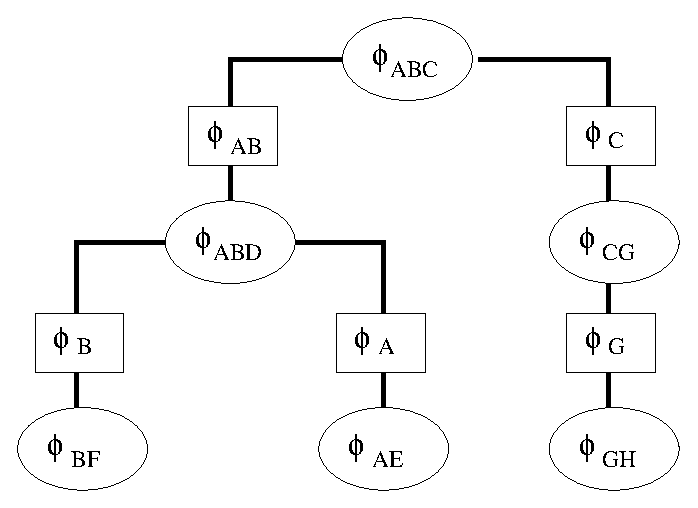
\includegraphics[width=100mm]{tree.eps}
    \caption{An example of a join tree}
    \label{fig2}
  \end{center}
\end{figure}

An example: the
variables are $\mathbf{U} = \{A, B, C, D, E, F, G, H\}$ and we have cliques
$C_1 = \{A, B, C\}$, $C_2 = \{A, B, D\}$, $C_3 = \{A, E\}$, $C_4 = \{B,
F\}$, $C_5 = \{C, G\}$, and $C_6 = \{G, H\}$. If we are interested in the
joint probability distribution of variables $\mathbf{V} = \{C, G, F\}$, it
can be calculated in the following way:
\begin{equation}
  \begin{split}
  P(\mathbf{V}) = \sum_A \phi_{ABC} &* \left[ \sum_D 
    \left( \frac{\phi_{ABD}}{\phi_{AB}}*
    (\sum_{\emptyset} \frac{\phi_{BF}}{\phi_{B}}) * 
    (\sum_E \frac{\phi_{AE}}{\phi_{A}}) \right) \right]\\
  &* \left[ \sum_{\emptyset} \left( \frac{\phi_{CG}}{\phi_C} * 
    (\sum_H \frac{\phi_{GH}}{\phi_G}) \right) \right].
  \end{split}
\end{equation}

As the example shows, the join tree is traversed in depth-first postorder
marginalising away all the variables which are not included in $V$ or the
current parent clique in the tree (see Fig.~\ref{fig2}). Again, the running
intersection property makes the algorithm straightforward.


\subsection{Functionality description}
The files \cfilename{clique.h} and \cfilename{clique.c} provide data 
types and functions for operating with sepsets and cliques. Together 
these form the concept known as join tree. In the NIP system, a join 
tree is merely an array of cliques which in turn have references to
all the necessary sepsets.

\subsubsection{The data structures}
\cfilename{clique.h} provides data types \cdatatype{sepset}, 
\cdatatype{sepset\_link}, and \cdatatype{clique}. \cdatatype{sepset}
is a pointer to a struct which has the following fields:
\begin{description}
\item[old] is older of the two last \cdatatype{potentials} passed via
the sepset.

\item[new] is the last \cdatatype{potential} passed via the sepset.

\item[variables] is an \cdatatype{array of variables}. These are the 
variables associated with the sepset. They are in the same order as
their cardinalities in the \cdatatype{potentials} \cstructfield{old} and 
\cstructfield{new}. Number of the variables can be found in either 
of the \cdatatype{potentials} \cstructfield{old} and \cstructfield{new}.

\item[cliques] is an \cdatatype{array of cliques}. The references to the
adjacent cliques are there. Size of the array is always two because of the
nature of sepsets.
\end{description}


The data type \cdatatype{sepset\_link} provides an implementation for lists
of \cdatatype{sepsets}. It is a pointer to a struct containing
\begin{description}
\item[data] which is a so-called \cdatatype{void pointer} because of the
  order of definitions. (You can't really define a list of sepsets before
  you have defined sepsets. sepsets can't be defined before cliques and
  cliques can't be defined before lists of sepsets.) When a list of
  sepsets is used, the \cstructfield{data} field has to be cast to the
  \cdatatype{sepset} type.

\item[fwd] which is the next \cdatatype{sepset\_link} in the list or 
  \cdatatype{NULL} at the end of the list.

\item[bwd] which is the previous \cdatatype{sepset\_link} in the list or 
  \cdatatype{NULL} at the beginning of the list.
\end{description}

The data type \cdatatype{clique} is a pointer to a struct containing all the
necessary information for working with cliques. The fields are
\begin{description}
\item[p] is the clique \cdatatype{potential}

\item[original\_p] is the original clique \cdatatype{potential} initialised
  according to the parameters of the model. This one is never affected 
  by the evidence entered into the model.

\item[variables] is an \cdatatype{array of variables}. These are the
  references to the variables associated with the clique. They are in
  the same order as their cardinalities in the 
  \cdatatype{potential}~\cstructfield{p}. The number of variables can be 
  found in the potential~\cstructfield{p}.

\item[sepsets] is a \cdatatype{sepset\_link} i.e. either
  \cdatatype{NULL} or a list of sepsets. The list contains the
  references to the adjacent sepsets.

\item[num\_of\_sepsets] is the number of adjacent sepsets.

\item[mark] is an \cdatatype{integer} used as a flag by various
  algorithms. For example a depth-first search and the propagation of 
  evidence uses the \cstructfield{mark} field to identify the cliques 
  which have already been handled.
\end{description}


\subsubsection{The functions}
The file \cfilename{clique.c} provides the following functions
\begin{description}
\item[make\_clique(vars, num\_of\_vars)] creates a \cdatatype{clique}. The
  associated variables are given as the \cdatatype{variable array}
  \cparameter{vars} and the number of the variables as the
  \cdatatype{integer} \cparameter{num\_of\_vars}. A shallow copy of the
  array is made, so remember to free it (but not the variables
  themselves). The clique will not have any adjacent sepsets
  initially: sepsets must be added separately.

\item[free\_clique(c)] frees the memory allocated by the 
  \cdatatype{clique}~\cparameter{c}. It will not free the memory allocated for 
  the corresponding \cdatatype{variables}, but all the adjacent 
  \cdatatype{sepsets} are freed and removed automatically so that rest
  of the join tree remains valid. Note that freeing an entire join tree
  can be done by calling this function for every clique.

\item[add\_sepset(c, s)] adds the \cdatatype{sepset} \cparameter{s} to the 
  \cdatatype{clique}~\cparameter{c}. Remember to add the sepset to both
  adjacent cliques and never add the same sepset to the same clique twice.

\item[make\_sepset(variables, num\_of\_vars, cliques)] creates a
  \cdatatype{sepset}. The associated variables are given as the
  \cdatatype{variable array} \cparameter{variables} and the size of the
  array as the \cdatatype{integer} \cparameter{num\_of\_vars}. Both
  adjacent cliques must be given as \cdatatype{array of cliques}
  (\cparameter{cliques}). This usually means that the \cdatatype{cliques}
  must be created before the \cdatatype{sepsets}. Note that a shallow copy
  of the parameter arrays is made, so freeing the arrays after calling the
  function is up to the user.
  
\item[free\_sepset(s)] just frees the memory allocated for the
  \cdatatype{sepset} \cparameter{s}. This is called automatically by 
  \cfunction{free\_clique} so usually this function is needed only for
  freeing possible useless \cdatatype{sepsets} which are not included in the 
  join tree.

\item[create\_potential(variables, num\_of\_vars, data)] can help if you
  need to create potentials out of \cdatatype{double arrays} like the
  \cparameter{data} parameter. The function creates a \cdatatype{potential}
  which has its data arranged correcty in order to work with the system. To
  rearrange the data correctly, the function needs to know the order of the
  corresponding variables. This is achieved by specifying the
  \cdatatype{variable array} \cparameter{variables} and the size of it as
  the \cdatatype{integer} \cparameter{num\_of\_vars}.

  The most important thing is to have the \cdatatype{variables} array in the 
  same order as the \cparameter{data} array is sorted. For example, the 
  potentials specified in the Hugin net language have the child variable
  as the least significant one: the value of the variable has the least 
  effect on the placement of the data. Thus the child variable should be 
  the first in the array. Note that for some reason the first parent 
  variable specified in the Hugin net language should be the last in 
  the \cparameter{variables} array, and the last parent should be the 
  second right after the child variable.

\item[unmark\_clique(c)] resets the mark in the 
  \cdatatype{clique}~\cparameter{c}. Note that this has to be done for 
  every clique before calling \cfunction{distribute\_evidence} or 
  \cfunction{collect\_evidence}.

\item[clique\_num\_of\_vars(c)] tells how many associated variables the 
  \cdatatype{clique}~\cparameter{c} has.

\item[sepset\_num\_of\_vars(s)] tells how many associated variables the 
  \cdatatype{sepset}~\cparameter{s} has.

\item[distribute\_evidence(c)] implements the algorithm which spreads 
  the evidence entered in to the cliques away from the given 
  \cdatatype{clique}~\cparameter{c}. See \cite{huang1994} page 21 for
  details. Remember to unmark all the cliques before calling this.

\item[collect\_evidence(c1, s12, c2)] implements the algorithm which
  collects evidence from the subtree rooted in the given
  \cdatatype{clique}~\cparameter{c2} and passes the evidence to the
  \cdatatype{clique}~\cparameter{c1}. The
  \cdatatype{sepset}~\cparameter{s12} is the sepset between the two
  cliques. The function is recursive and is usually used like this:
  \examplecode{collect\_evidence(NULL, NULL, c);} where \examplecode{c} is
  some \cdatatype{clique}. This causes the evidence to be collected from
  the entire join tree.  Remember to unmark all the cliques before calling
  this.

\item[gather\_joint\_probability(start, vars, n\_vars, isect, n\_isect)] is
  a recursive function for computing the joint probability distribution of 
  the \cparameter{n\_vars} variables contained by the \cdatatype{variable 
    array} \cparameter{vars}. The recursion begins (or continues) from the 
  \cparameter{start} \cdatatype{clique}.

  The \cparameter{isect} parameter is an \cdatatype{array of variables}
  containing the \cparameter{n\_isect} variables shared by the start and
  previous cliques. These are needed only for the recursion and the
  function is usually called like this:\\
  \examplecode{gather\_joint\_probability(c, vars, n, NULL, 0);} \\ where
  \examplecode{c} is some \cdatatype{clique} and \examplecode{vars}
  contains the \examplecode{n} variables of interest. The function returns
  a potential which is ordered accoding to the given variables, so the
  result depends on the order of \examplecode{vars} array.

% !!! NOTE !!! This requires variables to have a certain order in clique c!
\item[initialise(c, child, p, transient)] is used for entering the
  quantitative parameters of the model into the join tree. This function
  initialises the \cdatatype{clique}~\cparameter{c} with the given
  \cdatatype{potential}~\cparameter{p}. The initialisation ensures that the
  parameters are not reset by the \cfunction{global\_retraction} function,
  in case the \cparameter{transient} parameter is zero.  Note
  that~\cparameter{p} should be a valid \cdatatype{potential} i.e. the data
  contained by it should be correctly arranged and the number of variables
  specified in it should equal to the number of parent variables plus one
  (the child).
  
  Since the clique to be initialised can be associated with more
  variables than are associated with the potential, the user must
  specify the \cparameter{child} \cdatatype{variable}.

\item[marginalise(c, v, r)] is one of the most useful functions
  because it finds out the probability distribution of the 
  \cdatatype{variable}~\cparameter{v} according to the 
  \cdatatype{clique}~\cparameter{c} and writes it into the 
  \cdatatype{double array}~\cparameter{r} (as in \textbf{r}esult). 
  The array must be allocated before the function is called and the size 
  must be at least \examplecode{v->cardinality}. Note that the result is 
  NOT normalised.

\item[normalise(result, array\_size)] simply normalises the
  \cdatatype{double array} \cparameter{result}. After the function has
  executed, sum of the elements in the array will be one, unless it's
  filled with zeros. If the array is full of zeros, it is left
  unchanged. Size of the array must be specified as the \cdatatype{integer}
  \cparameter{array\_size}.

\item[global\_retraction(vars, nvars, cliques, ncliques)] resets the 
  clique potentials to the state they had after the initialisation and 
  enters the most recent evidence into the cliques. Thus the join tree
  consisting of the cliques is left at an inconsistent state and you may
  want to execute the global propagation consisting of 
  \cfunction{collect\_evidence} and \cfunction{distribute\_evidence}. 
  
  This function is needed for retracting evidence in some cases. To
  achieve this, the user must enter the wanted evidence into the
  variables and run \cfunction{global\_retraction}. The 
  \cdatatype{variable array} \cparameter{vars} (containing {\it all} the 
  variables) and a \cdatatype{clique array} \cparameter{cliques} must be 
  specified. Also number of the variables and cliques has to be given 
  to the function as the \cdatatype{integers} \cparameter{nvars}
  and \cparameter{ncliques}.

\item[enter\_observation(vars, nvars, cliques, ncliques, v, state)] 
  is made for incorporating hard evidence into a join tree. The observed
  state of the \cdatatype{variable}~\cparameter{v} is given as a 
  \cdatatype{string} named \cparameter{state}. The function needs also 
  the \cdatatype{variable array} \cparameter{vars}, 
  \cdatatype{clique array} \cparameter{cliques} and the size of them
  as the \cdatatype{integers} \cparameter{nvars} and \cparameter{ncliques}. 
  The reference \cparameter{vars} to the array of all variables is needed 
  because of the possible global retraction. The function 
  \cfunction{global\_retraction} is called automatically if needed.

\item[enter\_i\_observation(vars, nvars, cliques, ncliques, v, index)]
  is made for entering an observation as an \cdatatype{integer} into a join
  tree. This is equal to the function \cfunction{enter\_observation} but
  instead of telling the observation as a string, the user should encode
  the observation as the \cdatatype{integer} \cparameter{index}. A zero
  corresponds to the first state of the variable defined in the Hugin
  net language file. (See the \cfunction{get\_stateindex} function also.)

\item[enter\_evidence(vars, nvars, cliques, ncliques, v, evidence)]
  is made for entering soft evidence into a join tree. (Note that hard
  evidence is only a special case of soft evidence.) The function is
  similar to the \cfunction{enter\_observation} and
  \cfunction{enter\_i\_observation} functions above but instead of
  describing a single state, the user must specify a probability
  distribution as the \cdatatype{double array} \cparameter{evidence}. 
  The array is assumed to be normalised.
  
\item[find\_family(cliques, num\_of\_cliques, var)] finds a clique which
  contains the given variable \cparameter{var} and all of its parents. The
  set of cliques and size of the set must be specified as the parameters
  \cparameter{cliques} (\cdatatype{clique} array) and 
  \cparameter{num\_of\_cliques} (\cdatatype{integer}).

\item[find\_family\_mapping(family, child)] returns an \cdatatype{array of
  integers} which can be used as a mapping from the \cparameter{family} 
  \cdatatype{clique} to a potential containing the joint probability
  distribution of the family variables. The mapping array is useful with 
  the \examplecode{general\_marginalise} function.

\item[find\_clique(cliques, num\_of\_cliques, variables, num\_of\_vars)]
  tries to find a \cdatatype{clique} which contains all the variables (or
  more) specified in the \cdatatype{variable array}
  \cparameter{variables}. The number of variables has to be given as the 
  fourth parameter \cparameter{num\_of\_vars}. The function returns 
  \cdatatype{NULL} if there are no suitable cliques in the specified 
  \cdatatype{array of cliques} (\cparameter{cliques}) within the given 
  size \cparameter{num\_of\_cliques}. (remember to use find\_family 
  when possible, since it is faster due to memoization)

\item[find\_sepsets(cliques, num\_of\_cliques)] creates and inserts 
  the sepsets between the \cdatatype{cliques} specified in the array 
  \cparameter{cliques}. The size of the array must be given as the 
  \cdatatype{integer} \cparameter{num\_of\_cliques}. This function is 
  meant to be used only once after all the cliques have been created. 
  Consequently, it is not intended for repairing partially created 
  join trees.
  
\item[print\_clique(c)] is meant for debugging purposes. It prints the
  symbols of the variables associated with the
  \cdatatype{clique}~\cparameter{c} to the standard output.
  
\item[print\_sepset(s)] is meant for debugging purposes. It prints the
  symbols of the variables associated with the
  \cdatatype{sepset}~\cparameter{s} to the standard output.
  
\item[clique\_intersection(cl1, cl2, vars, n)] finds out which
  variables are common to the specified \cdatatype{cliques}~\cparameter{cl1}
  and~\cparameter{cl2}. The parameter \cparameter{vars} is a 
  \cdatatype{pointer to an array of variables} and the array will 
  contain the found variables  after the execution. Size of the
  array is written to the place pointed by the 
  \cdatatype{integer pointer}~\cparameter{n}. The resulting array
  is allocated by the function and it should be freed by the user.
\end{description}


\subsection{Other possibilities}
It could have been better to include the variables into the potential
datatype instead of the cliques. That way part of the duplicate bookkeeping
of variable cardinalities would have been avoided and potentials would be 
more ``independent'' entities. On the other hand, some parts of the system 
(like the time slice message passing) need to make potential operations as 
if they had different variables.

\newpage
\section{The Hugin net language parser}
\subsection{General}
The probabilistic models are defined using so-called {\it net language} 
developed by Hugin Expert A/S. Documentation about Hugin net language can 
be found at \\
\verb+http://developer.hugin.com/documentation/net/+
\footnote{Cited 14.7.2005}, but here is an introduction to the implemented
parser which is based on the first, a slightly restricted, revision of the 
language.

\subsubsection{Classes}
The parser assumes that each net file contains only one model which is
denoted as a {\it class} in net language. All the meaningful content
(i.e. not including whitespace nor comments) may optionally be enclosed in
a class statement. Such a statement begins with the keyword \textbf{class}
followed by the name of the model and the braces (\{ and \}) enclosing all
the other content. The implemented parser does not mind if the actual
content of the file is not enclosed in a class statement as long as there
are no extra braces, class keywords or otherwise incomplete definitions.

% inputs, outputs, node_size and other fields in net statement or not

\subsubsection{Nodes}

% statement

% label, position, states, NIP_next and other fields

\subsubsection{Potentials}

% statement

% Both structured and unstructured data fields...

% TODO...

\subsection{The functionality description}
The parser, for reading models from Hugin net language files, is
written in two files: \cfilename{huginnet.y} contains the lexer and 
description of the language for the Bison parser generator and 
\cfilename{parser.c} contains lots of helper functions for the parser. 
The data structures used for parsing are defined in the
\cfilename{parser.h} file. There's also a file named
\cfilename{fileio.c} which contains functions for tokenising the 
lines read from files.

\subsubsection{The data structures}
The \cfilename{parser.h} file defines several data types used with the
parser implementation. One of them is \cdatatype{doublelink} which is a
pointer to a struct which can hold a \cdatatype{double} and consequently
form a list of floating point numbers. The struct contains the
following fields
\begin{description}
\item[data] is the \cdatatype{double} number contained by the list element.

\item[fwd] is a \cdatatype{doublelink} i.e. a pointer to the next element in
the list or \cdatatype{NULL} at the end of the list.

\item[bwd] is a \cdatatype{doublelink} i.e. a pointer to the previous
element in the list or \cdatatype{NULL} at the beginning of the list.
\end{description}

Another kind of useful data type is \cdatatype{stringlink} which is a
pointer to a struct. The struct can be used as an element in a list of
strings. The element contains the following fields
\begin{description}
\item[data] is the \cdatatype{string} i.e. an array of characters.

\item[fwd] is a \cdatatype{stringlink} i.e. a pointer to the next element in
the list or \cdatatype{NULL} at the end of the list.

\item[bwd] is a \cdatatype{stringlink} i.e. a pointer to the previous
element in the list or \cdatatype{NULL} at the beginning of the list.
\end{description}

Since the conditional probability distributions and the structure of
the model are both encoded into the \examplecode{potential}
declarations of the net language, the distributions have to be 
temporarily stored until the entire net file has been parsed and the 
join tree is made. In other words, you can't enter the quantitative 
parameters of the model until you know the qualitative structure of
it. This is why the parser stores all the \cdatatype{potentials} read 
from the net file into a list until the end of parsing. This is where 
the data type \cdatatype{initDataLink} comes handy. It is a pointer to
a struct which holds the following fields
\begin{description}
\item[data] is the \cdatatype{potential} stored by the list element.

\item[child] is the \cdatatype{variable} which was defined to depend on
other variables in the potential declaration of the net language.

\item[parents] is an \cdatatype{array of variables} which contains the
parent variables of the \cstructfield{child}. Instead of an array it 
may be \cdatatype{NULL} if the \cstructfield{child} was an independent
variable and had no parents.

\item[fwd] is a pointer to the next element in the list or 
\cdatatype{NULL} at the end of the list.

\item[bwd] is a pointer to the previous element in the list or 
\cdatatype{NULL} at the beginning of the list.
\end{description}

A same kind of problem arises with the \examplecode{node} declarations 
of the Hugin net language when timeslices are defined. The parser 
can't assign the pointer from a \cdatatype{variable} to the 
corresponding \cdatatype{variable} in the next timeslice before both
of the variables have been parsed. This is solved by collecting the 
information about timeslice dependencies into a list until all the 
variables have been read from the net file. The file
\cfilename{parser.h} defines a data type for this purpose: 
\cdatatype{time\_init\_link} is a pointer to a struct which can be
used as an element in a linked list and holds the following fields
\begin{description}
\item[var] is the \cdatatype{variable} which corresponds
to another one in the next timeslice.

\item[next] is the symbol \cdatatype{string} which identifies the
corresponding variable in the next timeslice.

\item[fwd] is a \cdatatype{time\_init\_link} i.e. a pointer to the next
element in the list or \cdatatype{NULL} at the end of the list.
\end{description}

There's also a small parser for the data files. A data type has been
defined for reading timeseries data from files. The data type 
\cdatatype{datafile} is a struct which contains the following fields
\begin{description}
\item[name] is a string (\cdatatype{char array}) which contains the 
name of the file.

\item[separator] is the character (a single \cdatatype{char}) which is used 
as the separator between elements on a row in the data file.

\item[file] is a file handle of the type \cdatatype{FILE}.

\item[is\_open] is an \cdatatype{integer} telling whether the file is open
or not.

\item[firstline\_labels] is an \cdatatype{integer} which indicates whether
the first line of the data file contains node labels of the
corresponding variables or not. 

\item[line\_now] is an \cdatatype{integer} which tells the current position
in the file.

\item[datarows] is an \cdatatype{integer} telling the number of data rows in
the file i.e. the length of a timeseries. If there's a line containing
the node labels in the beginning of the file, it is not counted as a
data row.

\item[node\_symbols] is an \cdatatype{array of strings}. It contains the
symbols (short names) of the observed variables. These are usually
found on the first line of the data file.

\item[num\_of\_nodes] tells the number of the observed variables as an
\cdatatype{integer}.

\item[node\_states] is a \cdatatype{two-dimensional array of
strings}. It contains the names of the states of every observed
variable. For example \examplecode{node\_states[i][j]} is a name of a
state of the $i:th$ observed variable, assuming that $j \in [0, c-1]$, 
where $c$ is the cardinality of the variable. This array is
particularly useful if the model is created automatically from data
and not read from a net file.

\item[num\_of\_states] is an \cdatatype{array of integers} which tells how
many different states corresponding observed variable has had in the
data file.
\end{description}


\subsubsection{The functions}
The file created by Bison, \cfilename{huginnet.tab.c}, contains the
function which starts the Hugin net language file parser for reading a model
from a file.
\begin{description}
\item[yyparse()] must be included as an {\it external} function. 
(like \examplecode{extern int yyparse();}) It is the function which 
causes a model being parsed from a file. Use the helper functions at 
\cfilename{parser.c} to open the net language file prior to parsing, 
to close it after the execution and to dig out the newly created model.
\end{description}

For the sake of completeness, the lexer is described too. The file 
\cfilename{huginnet.y} contains the following function
\begin{description}
\item[yylex()] is used only by the parser created with Bison parser
generator. The function reads tokens from the input file, recognises
them and passes them to the parser appropriately.
\end{description}
It uses extensively the helper functions found in
\cfilename{fileio.c}. These are as follows
% fileio.c
\begin{description}
\item[count\_words(s, chars)] returns the number of words in the 
\cdatatype{string}~\cparameter{s}. The words are separated by white 
space and \cparameter{s} must be null terminated. If the 
\cdatatype{integer pointer} \cparameter{chars} is not a null pointer, 
the number of characters in~\cparameter{s} is written there.

\item[count\_tokens(s, chars, q\_strings, separators,
n\_separators, sep\_tokens, wspace\_sep)] counts the number of
tokens in the null terminated \cdatatype{string}~\cparameter{s}. The 
result is returned as an \cdatatype{integer}. The number of characters 
in the string is written to the integer referenced by the 
\cdatatype{integer pointer} \cparameter{chars}. 

Rest of the parameters make the function extremely versatile. The 
\cdatatype{integer} \cparameter{q\_strings} indicates whether possible
substrings enclosed in double quotes ('') should be considered as
single tokens or not. The \cdatatype{character array} 
\cparameter{separators} may be used for specifying additional
separators. Each character in the array behaves as a separator. 
A white space is always a separator. The number of the additional 
separators must be specified as the \cdatatype{integer} 
\cparameter{n\_separators}.

The \cdatatype{integer} \cparameter{sep\_tokens} is used as a flag 
to indicate whether the separators themselves should be considered as 
tokens or not. Finally, the \cdatatype{integer}
\cparameter{wspace\_sep} indicates whether white space should be 
considered as a separator token or just a plain separator.

\item[tokenise(s, n, q\_strings, separators, n\_separators, 
sep\_tokens, wspace\_sep)] is the tool for finding \cparameter{n} first 
tokens in the null terminated \cdatatype{string}~\cparameter{s}. The 
function returns an \cdatatype{array of integers} which tells where 
each token begins and where they end. The first integer in the array 
tells which character in the string begins the first token. The second
integer tells the place of the first character NOT included in the
first token. The third and fourth integers tell the placement of the
second token and so on.

Rest of the parameters are similar to the ones in the 
\cfunction{count\_tokens} function. The \cdatatype{integer} 
\cparameter{q\_strings} indicates whether we want quoted strings to 
be single tokens or not. The \cdatatype{character array} 
\cparameter{separators} specify separators in addition to white space 
and the \cdatatype{integer} \cparameter{n\_separators} tells the 
number of additional separators. The \cdatatype{integer} 
\cparameter{sep\_tokens} indicates whether we want the
separators to be tokens as well. If the \cdatatype{integer}
\cparameter{wspace\_sep} is not zero, the white space will behave as
separator but will not be considered as a token even if the other
possible separators are.

\item[split(s, indices, n)] uses the \cdatatype{integer array}
\cparameter{indices} (made by the \cfunction{tokenise} function) to
split the null terminated \cdatatype{string}~\cparameter{s} into 
\cparameter{n} strings. The function returns the strings as an array. 
(\cdatatype{char**} i.e. an array of character arrays)
\end{description}


Most of the actions executed by the net language file parser is done by the
functions in \cfilename{parser.c}. The functions are as follows
\begin{description}
\item[open\_yyparse\_infile(filename)] is one of the most important
functions in reading models from files. It opens a file for the parser
for reading and returns zero if the file was opened successfully. The 
name of the file is given as the \cdatatype{string} \cparameter{filename}.

\item[close\_yyparse\_infile()] should be called after parsing a model
from a file. It closes the net language file appropriately.

\item[open\_datafile(filename, separator, write, nodenames)] is used
for opening data files for reading or writing. The function returns a 
pointer to the created \cdatatype{datafile} struct. The name of the data
file is given as the \cdatatype{string} \cparameter{filename} and the used
separator is given as the \cdatatype{character}
\cparameter{separator}. The \cdatatype{integer} \cparameter{write} is used
for indicating whether the file should be opened for reading only
(zero) or for writing only (non-zero). The \cdatatype{integer} flag
\cparameter{nodenames} tells the function to treat the first line of
the file as regular data (zero) or use the tokens on the line as the 
symbols of the variables. If \examplecode{nodenames == 0} the function 
invents its own symbols for the variables to be included with the 
\cdatatype{datafile} struct.

\item[close\_datafile(file)] closes the data file included in the
given \cdatatype{datafile pointer} \cparameter{file} and frees the memory
allocated for the \cdatatype{datafile} struct.

\item[nextline\_tokens(f, separator, tokens)] is the function made for
reading data files. It reads the next line of the \cdatatype{datafile}
referenced by the pointer~\cparameter{f} and splits the line into
tokens. The separator should be specified as the \cdatatype{character}
\cparameter{separator}. The function returns the number of tokens as an 
\cdatatype{integer} and sets the pointer \cparameter{tokens} to
reference the resulting \cdatatype{array of strings}. I.e. 
\cparameter{tokens} is a pointer to an array of character arrays, or
in other words a \examplecode{char***}. Make sure that you don't lose 
any existing pointers by calling this function, because freeing the 
tokens read from the file is up to the user.

\item[next\_token(token\_length)] is used by the net language
parser. The function returns the next token from the opened net file
and writes the length of the token to the \cdatatype{integer} referenced by
the pointer \cparameter{token\_length}. The token is a (null terminated)
\cdatatype{string} i.e. an array of characters. The token length does not
include the NULL character and equals zero if there are no more tokens
in the file. After the token string has been used, please free the
memory allocated for it.

\item[add\_symbol(v)] is used only by the net language parser. The
function adds the \cdatatype{variable}~\cparameter{v} into a temporary 
list of parent variables. The list is needed for parsing the parent 
variables according to the potential declarations of the net
language. (See also the \cfunction{make\_variable\_array} function)

\item[add\_initData(p, child, parents)] is used only by the net
language parser. This function adds the parsed 
\cdatatype{potential}~\cparameter{p}, the \cdatatype{variable} 
\cparameter{child} and its \cparameter{parents} in an 
\cdatatype{array of variables} to the list of parsed potentials. 
The potentials are collected into the list until the join tree has
been created and it can be initialised with the potentials.

\item[add\_time\_init(var, next)] is used only by the net language
parser. It adds information about the correspondence of nodes between
timeslices into a temporary list. The \cdatatype{variable}
\cparameter{var} will correspond to the \cdatatype{variable}
identified by the symbol \cdatatype{string} \cparameter{next} in the 
next timeslice. The information has to be collected into a list,
because the another variable may haven't been created yet at the
moment. After the variables have been parsed, the list is cleaned.

\item[add\_double(d)] is used only by the net language parser. The
function adds the \cdatatype{double}~\cparameter{d} into a temporary list of
floating point numbers. Usually the list is used for storing the
numbers of the data fields of the potential declarations in the net
files. The list can be turned into an array by the
\cfunction{make\_double\_array} function.

\item[add\_string(string)] is used only by the net language
parser. Calling this function will add the null terminated \cdatatype{array
of characters} \cparameter{string} into a temporary list. The list is used
for storing the names of the states declared in the node declarations
of the net language. The list can be turned into an array by using the
\cfunction{make\_string\_array} function.

\item[make\_variable\_array()] is used only by the net language
parser. The function creates an array containing the \cdatatype{variables}
accumulated in the temporary list by \cfunction{add\_symbol}
function. The resulting array is usually used as the array of parent 
variables.

\item[make\_double\_array()] is used only by the net language
parser. It creates an \cdatatype{array of doubles} containing the numbers
accumulated into the temporary list by the the \cfunction{add\_double}
function. The array is used as the data for the parsed potentials. 

\item[make\_string\_array()] is used only by the net language
parser. The function creates an \cdatatype{array of strings} out of the list
created by the \cfunction{add\_string} function. The array is used as the
statename array of the parsed variables.

\item[reset\_doubles()] cleans the temporary list of floating point
numbers created with the \cfunction{add\_double} function. The function
should be used only by the net language parser.

\item[reset\_strings()] cleans the list of \cdatatype{strings} gathered with
the \cfunction{add\_string} function. This function does NOT free the
actual strings, only the list structure. The function is meant to be
used only by the net language parser.

\item[reset\_symbols()] cleans the temporary list of variables made by
the \cfunction{add\_symbol} function. The function does NOT free the
actual \cdatatype{variables}, only the list structure itself. It is meant to
be used only by the net language parser.

\item[reset\_initData()] cleans the data used for initialising the
join tree. The function also frees the \cdatatype{potentials} and the arrays of
parent \cdatatype{variables} gathered in the list. (The variables themselves
are not freed, of course.) The function is meant to be used only by
the net language parser.

\item[reset\_timeinit()] cleans the temporary list about the timeslice
correspondencies accumulated by the \cfunction{add\_time\_init} function.
Only the list structure and the stored symbol string are freed, not
the referenced variables. The function is meant to be used only by the
net language parser.

\item[init\_new\_Graph()] is meant to be used only by the net language
parser. The function initialises a new \cdatatype{Graph} which can hold as
many variables than is parsed from the file so far.

\item[parsedVars2Graph()] executes one stage in the net language
parser. It inserts the \cdatatype{variables} into the initialised
\cdatatype{Graph} after all of the variables have been created. The
function adds also the child-parent relation to the
\cdatatype{Graph}. Therefore it must be called after all of the
\verb+potential+ declarations of the net file have been parsed and the
information can be found from the initialisation list accumulated by
the \cfunction{add\_initData} function.

\item[time2Vars()] is used only by the net language parser. The
function adds the information about the correspondence of variables
between timeslices to the \cdatatype{variables}. The procedure must be
executed after all of the \examplecode{node} declarations of the net 
language file have been parsed. It uses the information gathered into the
temporary list created by the \cfunction{add\_time\_init} function.

\item[Graph2JTree()] creates a join tree from the \cdatatype{Graph} made by
the previous functions. This function is to be executed only by the
net language parser. After the \cdatatype{cliques} (and 
\cdatatype{sepsets}) have been created, the procedure frees the memory 
used by the graph.

\item[parsedPots2JTree()] is meant to be used only by the net language
parser. The function initialises the cliques created by the previous
functions and uses the \cdatatype{potentials} collected into the temporary
list by the \cfunction{add\_initData} function. Thus the parameters of the
model will be entered into the data structure.

\item[print\_parsed\_stuff()] is meant only for debugging purposes. It
prints the potentials parsed by the net language parser to the
standard output. The function uses the information collected into the 
temporary list by the \cfunction{add\_initData} function.

\item[set\_nip\_statenames(states)] is used only by the net language
parser. It sets a temporary pointer to the \cdatatype{string array}
\cparameter{states}. 

\item[get\_nip\_statenames()] is used only by the net language
parser. It gets the temporary pointer to the \cdatatype{string array}
set by the previous function. 

\item[set\_nip\_label(label)] is used only by the net language
parser. It sets a temporary pointer to the \cdatatype{string}
\cparameter{label}.

\item[get\_nip\_label()] is used only by the net language
parser. It gets the temporary pointer to the \cdatatype{string}
set by the previous function.

\item[set\_nip\_next(next)] is used only by the net language
parser. It sets a temporary pointer to the \cdatatype{string}
\cparameter{next}.

\item[get\_nip\_next()] is used only by the net language
parser. It gets the temporary pointer to the \cdatatype{string}
set by the previous function.

\item[get\_nip\_symbols\_parsed()] returns the number of parent
variables when parsing a \examplecode{potential} declaration of a net
language file. It is meant to be used by the net language parser only.

\item[get\_nip\_strings\_parsed()] returns the number of states when
parsing a \examplecode{node} declaration of a net language file. It is
meant to be used by the net langugage parser only.

\item[get\_num\_of\_cliques()] is to be used for getting the number of
cliques created by the parser. This is one of the functions for
finding out the results of parsing a net language file. (See also the
other functions: \cfunction{get\_cliques\_pointer} and
\cfunction{reset\_clique\_array}) 

\item[get\_cliques\_pointer()] gets you a pointer to the \cdatatype{array of
cliques} created by the net language parser. (I.e. the returned value
is a \cdatatype{clique**})

\item[reset\_clique\_array()] resets the net language parser so that
it can read more net language files. Call this function after you have
discovered the number and location of cliques. Freeing the memory
allocated by the join tree created by the parser is up to the user: 
just use the \cfunction{free\_clique} function for every clique in the array
when the join tree becomes useless.

\end{description}


\subsection{Other possibilities}

How the stuff could work also...


\newpage
\section{The NIP and timeslice handler} 
% Some system which handles time series?

\subsection{General}

The idea and mathematical formulas...

\subsection{The functionality description}

The interface + how the stuff works...

\subsection{Other possibilities}

How the stuff could work also...
% a tree of variables instead of an array?


\newpage
\chapter{System analysis}
% The cost of using it
\section{The parser}

\section{The graph}
The underlying assumptions with the \cdatatype{Graph} have been the following:
\begin{enumerate}
\item The graphical analysis step will only be run once per graph.
\item The number of variables in a graph will be relatively small.
\end{enumerate}

The analysis is divided into two blocks. First we study operations
that modify the Graph, and then follow with a discussion of the
cluster/clique-building phase. These two stages use very different
data structures and algorithms, which makes unified analysis
difficult.

The first graphical operation is the creation of the graph
itself. This is a relatively simple operation and for all practical
purposes constant time. Adding new variables is also constant time per
variable. After all variables have been added, the internal
datastructures are sorted with standard C library quicksort. This
incurs an $O(n \log n)$ penalty. However, it is run only once per
graph and the implementation is quite efficient.

Of the purely graphical operations, moralisation dominates others by
an order of magnitude. Since the operations are done on a copy of the
original graph, we should also consider those costs. However, it turns
out that creating a copy of the graph is at most $O(n^2)$ operation
and thus also dominated by moralisation. Furthermore, most operations
are implemented using \cfunction{memcpy} which should guarantee
almost optimal performance on a given platform.

The moralisation step itself is an $O(n^3)$ operation. For each of the
$n$ variables we have potentially $(n-1)(n-2)/2$ possible pairs of a
child and a parent. Like all graphical operations, it is run only once
per graph and should not be a bottleneck in most applications.

Technically the triangulation operation is also a graphical
operation. Since it is more complex than the previous operations and
outputs cliques, it is analysed separately.

Building the heap required in the triangulation step is $O(n \log
n)$. This cost is neglible compared to the actual cluster building
loop, in which we iterate through every $n$ variable. A short outline
of the operations performed in the loop follows.

The most timeconsuming operation is the extraction of the minimum
algorithm. Superficially it is only a $O(k log n)$ operation as
mentioned in the XXX. Because we have to dynamically update the 



% Create a heap based on the moral graph.
% Extract $n$ clusters from the heap.
% Check if the cluster is a subset of a previously found clique.
% Add to the 

% Vois olla, ett� heapin buildaus olis n log n?
% N�ytt�isi silt�, ett� trianguloinnissa tehd��n n kertaa looppi:
% T�ss� loopissa tehd��n yksi kappale extract_mini� (joka on k log n?)
% h�psis, clean_item vie t�yden k rundia, eli nnk
% no onpa vaikea.
% sit yks k^2 -looppi (matriisin asettelu)
% ja lopulta is_subset: n*n*k?

%clique building


\section{The join tree}

\section{The timeslice-monster}


%\newpage
%\chapter{Comments}


\newpage
\appendix
\renewcommand{\thesection}{A-\arabic{section}}
% redefine the command that creates the equation no.
\setcounter{section}{0}  % reset counter 
\section*{APPENDIX}  % use *-form to suppress numbering


\section{Net language example}
\VerbatimInput{example.net}

\newpage
\bibliography{doc}

\end{document}
